%%%%%%%%%%%%%%%%%%%%%%%%%%%%%%%%%
% This is a slightly modified template of the one built by
% Steven V. Miller. Information can be found here:
%  http://svmiller.com/blog/2016/02/svm-r-markdown-manuscript/
%
% I added the use of raggedright to the anonymous option
% because journals,  the ability to put all the footnotes
% in endnotes, and the ability to manually adjust
% the starting page from the YAML header.
%
% Here are the options that you can define in the YAML
% header.
%
% fontfamily - self-explanatory
% fontsize - self-explanatory (e.g. 10pt, 11pt)
% anonymous - true/false. If true, names will be supressed and the
%                       text will be double-spaced and ragged
%                       right. For submission. 
% endnotes - true/false. If true, the footnotes will be put in a
%                   section at the end just ahead of the references.  
% keywords - self-explanatory
% thanks - shows up as a footnote to the title on page 1
% abstract - self explanatory
% appendix - if true, tables and figures will have  in
%                   front
% appendixletter - The letter to append to tables and figures in
%                             appendix
% pagenumber - Put in a number here to get a starting page number
%                         besides 1. 
%%%%%%%%%%%%%%%%%%%%%%%%%%%%%%%%%%


\documentclass[11pt,]{article}
\usepackage[left=1in,top=1in,right=1in,bottom=1in]{geometry}
\usepackage{amsmath}
\usepackage{float}
\usepackage{dcolumn}

\newcommand*{\authorfont}{\fontfamily{phv}\selectfont}
\usepackage[]{mathpazo}


  \usepackage[T1]{fontenc}
  \usepackage[utf8]{inputenc}



\usepackage{abstract}
\renewcommand{\abstractname}{}    % clear the title
\renewcommand{\absnamepos}{empty} % originally center

\providecommand{\tightlist}{%
  \setlength{\itemsep}{0pt}\setlength{\parskip}{0pt}}

\renewenvironment{abstract}
 {{%
    \setlength{\leftmargin}{0mm}
    \setlength{\rightmargin}{\leftmargin}%
  }%
  \relax}
 {\endlist}

\makeatletter
\def\@maketitle{%
  \newpage
%  \null
%  \vskip 2em%
%  \begin{center}%
  \let \footnote \thanks
    {\fontsize{18}{20}\selectfont\raggedright  \setlength{\parindent}{0pt} \@title \par}%
}
%\fi
\makeatother




\setcounter{secnumdepth}{0}


\usepackage{graphicx}
% We will generate all images so they have a width \maxwidth. This means
% that they will get their normal width if they fit onto the page, but
% are scaled down if they would overflow the margins.
\makeatletter
\def\maxwidth{\ifdim\Gin@nat@width>\linewidth\linewidth
\else\Gin@nat@width\fi}
\makeatother
\let\Oldincludegraphics\includegraphics
\renewcommand{\includegraphics}[1]{\Oldincludegraphics[width=\maxwidth]{#1}}

\title{Are Women Actually Better Doctors? The Relationship Between Female
Physicians and Maternal Mortality Ratios \thanks{Thanks to Dr.~Aaron Gullickson for putting up with my complete lack of
knowledge in both statistics and R. Your patience is appreciated. I will
not miss feeling like a complete idiot every Tuesday and Thursday.}  }



\author{\Large Olivia Atkinson\vspace{0.05in} \newline\normalsize\emph{University of Oregon, Political Science}  }


\date{}

\usepackage{titlesec}

\titleformat*{\section}{\normalsize\bfseries}
\titleformat*{\subsection}{\normalsize\itshape}
\titleformat*{\subsubsection}{\normalsize\itshape}
\titleformat*{\paragraph}{\normalsize\itshape}
\titleformat*{\subparagraph}{\normalsize\itshape}


\usepackage{natbib}
\bibliographystyle{./resources/ajs.bst}


%\renewcommand{\refname}{References}
%\makeatletter
%\renewcommand\bibsection{
%    \section*{{\normalsize{\refname}}}%
%}%
%\makeatother

\newtheorem{hypothesis}{Hypothesis}
\usepackage{setspace}

\makeatletter
\@ifpackageloaded{hyperref}{}{%
\ifxetex
  \usepackage[setpagesize=false, % page size defined by xetex
              unicode=false, % unicode breaks when used with xetex
              xetex]{hyperref}
\else
  \usepackage[unicode=true]{hyperref}
\fi
}
\@ifpackageloaded{color}{
    \PassOptionsToPackage{usenames,dvipsnames}{color}
}{%
    \usepackage[usenames,dvipsnames]{color}
}
\makeatother
\hypersetup{breaklinks=true,
            bookmarks=true,
            pdfauthor={Olivia Atkinson (University of Oregon, Political Science)},
             pdfkeywords = {maternal mortality, female physicans, gender norms and behavior},  
            pdftitle={Are Women Actually Better Doctors? The Relationship Between Female
Physicians and Maternal Mortality Ratios},
            colorlinks=true,
            citecolor=blue,
            urlcolor=blue,
            linkcolor=magenta,
            pdfborder={0 0 0}}
\urlstyle{same}  % don't use monospace font for urls

\usepackage{endnotes}


\newlength{\normalparindent}
\setlength{\normalparindent}{\parindent}

%prettier captions for figures and tables
%I am making the text of figure captions smaller but not table captions
\usepackage[labelfont=bf,labelsep=period]{caption}
\captionsetup[figure]{font=footnotesize}

\begin{document}
	
% \pagenumbering{arabic}% resets `page` counter to 1 
%
\setcounter{page}{1}

% \maketitle

{% \usefont{T1}{pnc}{m}{n}
\setlength{\parindent}{0pt}
\thispagestyle{plain}
{\fontsize{18}{20}\selectfont\raggedright 
\maketitle  % title \par  

}

{
   \vskip 13.5pt\relax \normalsize\fontsize{11}{12} 
\textbf{\authorfont Olivia Atkinson} \hskip 15pt \emph{\small University of Oregon, Political Science}   

}

}





\vskip 6.5pt

\noindent  \section{Introduction}\label{introduction}

Maternal mortality rates in the United States are among some of the
highest in developed countries. In other developed countries maternal
mortality rates have been steadily falling, while rates in the U.S. are
continuing to rise. This seems especially troubling for a country like
the United States where access to care and treatment is and should be
easy, hypothetically. However, while the U.S. as a whole has access to
some of the best medical resources in the world, only a certain portion
of the population are able to access those resources and the care that
they need.

Additionally, maternal mortality rates are hard to calculate and
accurately record. Although the rising rates of maternal mortality are
caused by a myriad of reasons ranging from the increasing age of mothers
to more structural issues like a broken and complicated healthcare
system it should not deter reserachers from conducting research that can
better uncover the reasons (even if they are multiple) leading to the
alarming rise of maternal deaths. In fact, the lack of data and the
difficulty of conducting such research should be a motivating factor for
other researchers and scholars who are invested in finding underlying
causes of maternal deaths and suggesting policy solutions to help
alleviate them.

Another trend that has been on the rise in the United States is the
percentage of female physicians. Today, the majority of physicians under
the age of 35 are women (M. Johnson 2018). With the number of female
physicians on the rise, I am interested in looking at the relationship
between the maternal mortality ratios and the percentage of patients who
see female doctors. The main question this paper seeks to answer is:
Does seeing a female physician decrease a woman's chances of dying from
pregnancy related causes? Because of gendered norms and behavior, women
are thought to be and generally are more caring, attentive, and
emotionally available compared to their male counterparts who are seen
as aggressive, unwelcoming, and less communicative. This translates in a
number of areas in social life, and this paper is interested in seeing
if it would also transfer into the medical profession, as well.

There have been a number of studies conducted that look at the
relationship between patient care and physician gender (C. Y. Johnson
2016, Berthold, et. al. 2008, Tsugawa et. al. 2017). However, none of
the studies have looked specifically at a physician's gender and its
relationship to maternal mortality. As such, this project hopes to fill
a gap in the literature and also encourage further studies that look at
this specific relationship.

\section{Data and Methods}\label{data-and-methods}

Data on maternal mortality and natality was collected from the CDC
WONDER database. WONDER is an acronymn for Wide-ranging Online Data for
Epidemiologic Research and provides public health data and information
to the public. The maternal mortality ratio was calculated by dividing
the total number of maternal deaths in a census region by the total
number of births in a census region from the years 2000-2016.

The data for ``Detailed Mortality - Underlying Cause of Death''" is
based on death certificates for U.S. residents. The detailed mortality
data is compiled from data provided by the 57 vital statistics
jurisdictions through the Vital Statistics Cooperative. The data set is
produced by the U.S. Department of Health and Human Services, Centers
for Disease Control and Prevention, National Center for Health
Statistics, and the Division of Vital Statistics, Mortality Statistics
Branch. (\url{https://wonder.cdc.gov/DataSets.html}). The natality data
is the number of live births occurring within a given year. The natality
data is divided up into three databases (1995-2002, 2003-2006, and
2007-2017) because of changes in reporting standards regarding race in
2003.

Data for physician gender was taken from the IPUMS Health Surveys in the
Medical Expenditure Panel Survey. The MEPS is a survey conducted through
five rounds of interviews over a period of roughly two years. The data
for physician gender reports whether the individual's usual source of
care provider is male or female. To be asked the question about their
physician's gender, survery respondents had to be eligible for the
Access to Care supplement. To be eligible, individuals had to be
current, non-institutionalized members of the responding unit in round 2
for panel members in relative year 1 and round 4 for panel members in
relative year 2.

In the maternal mortality dataset I created a subset of the region,
year, and deaths variables. In the natality dataset I created a subset
of region, year, and births variables. I then created the maternal
mortality ratio by first merging the maternal deaths data with the
births data then divided deaths by births. For the data on physician
gender, I dropped all responses that were male, unknown, or coded ``not
in universe''. From there, I subset the female physician data by year
and region. Finally, I merged the maternal mortality ratio data with the
percent female doctor data.

The data for maternal deaths were only available at the census region
level. Thus, the results and any analysis drawn from the results are
very crude. Also, the data on a individual's physician's gender was
self-reported and only certain people were eligible to answer the
question. However, this still provides a good starting point for further
research on this topic. The data is also limited because no other
independent variables were controlled for in such as age, income, etc.
However, I felt it was unnecessary to include these variables since I
was working on such an abstracted level (i.e.~census region). If this
project was conducted on the state level, other variables such as the
ones previously listed would be useful to include in the analysis.

I used a two-way fixed effects OLS regression analysis that used within
fixed effects for census region and year. This allowed me to rule out
spuriousness from the time-constant covariates of percent female and
maternal mortality. Because both of these trends have been steadily
rising over the years, it seemed as though as the number of female
physicians increased so did the maternal mortality ratio, disproving my
hypothesis. However, once I put in dummy variables for year the
relationship between female physicians and maternal mortality changed to
now show a positive effect between increased rates of female physicians
and maternal mortality rates. In other words, as the percentage of
female physicians went up, the maternal mortality ratio decreased. I
also included a dummy variable for region to soak up any within region
differences that might be accounting for a change in maternal mortality
rates to get a better look at the relationship between physician gender
and maternal mortality rates.

The first figure is a bivariate graph that shows the relationship
between the percentage of female physicians with maternal mortality
rates without accounting for the simultaneous increase over the years. I
multiplied the the maternal mortality ratio by 100,000 in the first and
second graph because the numbers were small therefore making the graph
more easily understandable. The second and third figures separate out
the maternal mortality ratio and the percentage of female physicians by
year to show that each is increasing.

The models I ran are OLS two-way within fixed effects regression tables.
The only model of particular importance for this study is Model 4, which
is the two-way fixed effects model with dummy variables for both region
and year.

\section{Results}\label{results}

Figure 1 is a bivariate graph that shows the maternal mortality ratio by
percent female physicians. As you can see, in every census region as the
percent of female doctors increases so does the maternal mortality
ratio. This is exactly opposite of the expected results based on priors
and outside literature. Figure 2 and Figure 3 are both bivariate graphs
showing that maternal mortality and the percent of female doctors has
been increasing over the years. Because both maternal mortality rates
and the percentage of female doctors have been increasing when looking
at the relationship together it seems as though an increase in the
percent of female doctors correlates to an increase in maternal deaths.

This relationship is shown in the regression table, as well. Model 2
shows the maternal mortality ratio by percent female doctor. For every
one percent increase in female doctors there is a .2 percent increase in
the maternal mortality ratio, on average.

However, as Model 4 shows when the year and region are fitted with dummy
variables the relationship between the percentage of female physicians
and the maternal mortality ratio flips. The maternal mortality ratio
actually decreases as the percentage of female physicians increases.
However, this relationship is not statistically significant. On average,
for every one percent increase in female physicians there is a 1.6
percent decrease in the maternal mortality ratio. While this does not
seem that significant, as mentioned above in the data section, this data
is at the census region level so any analysis or results will be
somewhat crudely generalizable.

Although the R-squared values are significant, this is a fixed effects
model so the R-squared values are basically meaningless because they
include all of the time-constant variation making them inaccurate.

Looking at the data by region, it becomes clear that there are major
disparities between regions, especially the South and the West. As shown
in Figure 2, the West has the lowest number of maternal deaths and the
South has the most. The Midwest and Northeast are relatively similar. In
Figure 3, the South has the lowest percentage of female physicians
whereas the West has the highest. Again, the Midwest and the Northeast
are relatively similar in the middle.
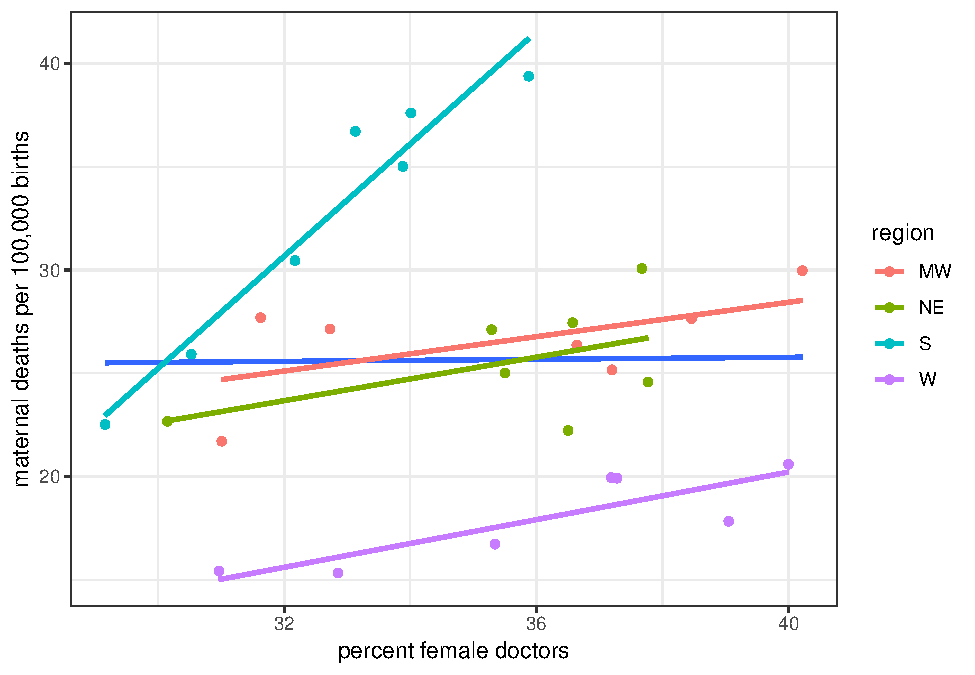
\includegraphics{main_files/figure-latex/name1-1.pdf}

\begin{figure}
\centering
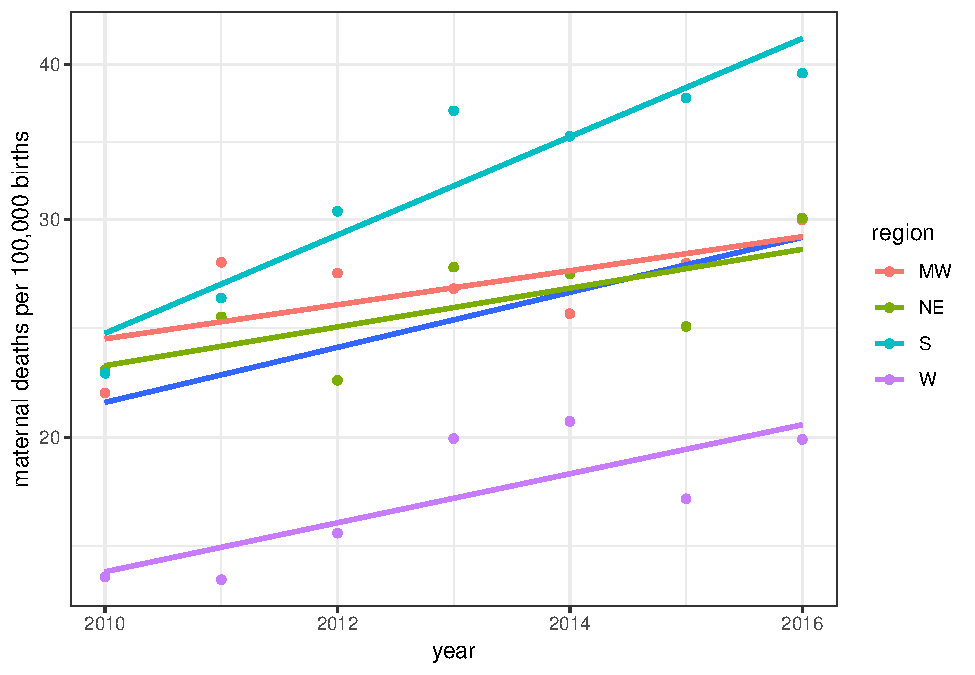
\includegraphics{main_files/figure-latex/name2-1.pdf}
\caption{maternal mortality ratio by year}
\end{figure}

\begin{figure}
\centering
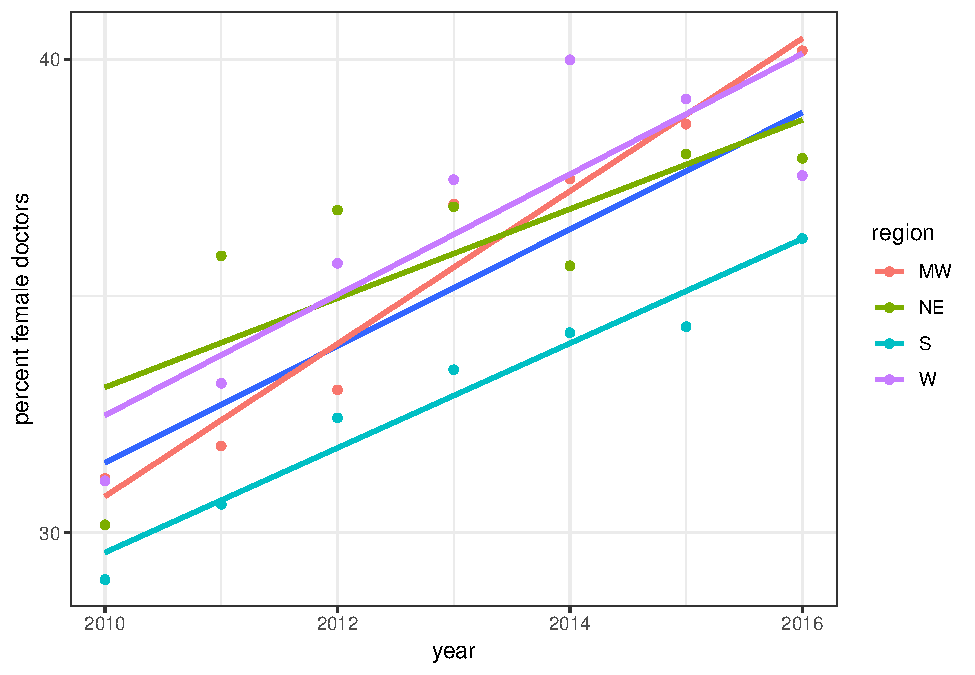
\includegraphics{main_files/figure-latex/name3-1.pdf}
\caption{percent female physicians by year}
\end{figure}

\begin{table}
\caption{Regression Model Predicting Maternal Mortality Ratios by Percent Female Doctors}
\begin{center}
\begin{tabular}{l c c c c }
\hline
 & Model 1 & Model 2 & Model 3 & Model 4 \\
\hline
(Intercept)         & $-8.441^{***}$ & $-8.383^{***}$ & $-9.394^{***}$ & $-7.960^{***}$ \\
                    & $(0.054)$      & $(0.557)$      & $(0.263)$      & $(0.469)$      \\
regionNE            & $-0.037$       &                & $-0.044$       & $-0.033$       \\
                    & $(0.048)$      &                & $(0.057)$      & $(0.048)$      \\
regionS             & $0.190^{***}$  &                & $0.279^{***}$  & $0.147^{*}$    \\
                    & $(0.048)$      &                & $(0.061)$      & $(0.063)$      \\
regionW             & $-0.392^{***}$ &                & $-0.414^{***}$ & $-0.381^{***}$ \\
                    & $(0.048)$      &                & $(0.058)$      & $(0.049)$      \\
as.factor(year)2011 & $0.119$        &                &                & $0.155^{*}$    \\
                    & $(0.064)$      &                &                & $(0.073)$      \\
as.factor(year)2012 & $0.147^{*}$    &                &                & $0.207^{*}$    \\
                    & $(0.064)$      &                &                & $(0.086)$      \\
as.factor(year)2013 & $0.283^{***}$  &                &                & $0.370^{**}$   \\
                    & $(0.064)$      &                &                & $(0.106)$      \\
as.factor(year)2014 & $0.264^{***}$  &                &                & $0.362^{**}$   \\
                    & $(0.064)$      &                &                & $(0.114)$      \\
as.factor(year)2015 & $0.245^{**}$   &                &                & $0.354^{*}$    \\
                    & $(0.064)$      &                &                & $(0.124)$      \\
as.factor(year)2016 & $0.355^{***}$  &                &                & $0.471^{**}$   \\
                    & $(0.064)$      &                &                & $(0.129)$      \\
percent\_female     &                & $0.002$        & $0.033^{***}$  & $-0.016$       \\
                    &                & $(0.016)$      & $(0.007)$      & $(0.015)$      \\
\hline
R$^2$               & 0.915          & 0.001          & 0.847          & 0.920          \\
Adj. R$^2$          & 0.873          & -0.038         & 0.820          & 0.873          \\
Num. obs.           & 28             & 28             & 28             & 28             \\
RMSE                & 0.090          & 0.258          & 0.107          & 0.090          \\
\hline
\multicolumn{5}{l}{\scriptsize{$^{***}p<0.001$, $^{**}p<0.01$, $^*p<0.05$}}
\end{tabular}
\label{table:coefficients}
\end{center}
\end{table}

\section{Conclusions}\label{conclusions}

In conclusion, this project looked at how the percentage of female
physicians effected the maternal mortality rate. The data tells us that
the percentage of female physicians has an effect on maternal mortality
ratios. While these results were not statistically significant, I
hypothesize that better data at a smaller unit of analysis will show
similar but stronger results. As such, further research should be
conducted regarding this issue.

As stated previously, the results drawn from this study are crude at
best. However, it does offer a starting point for other more in-depth
research on the relationship between maternal mortality ratios and the
gender of a patient's physician. This obviously should not discourage
men from practicing medicine. However, it should highlight how engrained
gender ideas, norms, and behaviors can have real-world effects. Male
physicians should be more aware of how they interact with patients and
take more care to listen to their patients, ask them how they feel about
the care they are getting, discussing care adn treatment options openly
with patients as well as being more open to engaging in conversation and
welcoming questions and comments from patients throughout the process.

On a larger scale, this points to how harmful gendered norms and
behavior can be, not only for individual people but for those they
interact with, too. Working to dismantle these stereotypes and
expectations from a young age will have large-scale effects in the long
run.

Any studies on maternal mortality and its underlying causes should be
taken seriously as it is a trend in the United States that is
increasing. The health and wellness of women is something that, as we
have seen recently, is not taken seriously by certain governmental
bodies. Further, there should be more research conducted to understand
the differences between regional differences of maternal mortality and
what can be done to alleviate those causes. The South is a rural area
and many women do not have immediate access to the care that they need
pre- and post-natal.

\section{References}\label{references}

Berthold, H. K., Gouni‐Berthold, I. , Bestehorn, K. P., Böhm, M. and
Krone, W. (2008), Physician gender is associated with the quality of
type 2 diabetes care. Journal of Internal Medicine, 264: 340-350.
\url{doi:10.1111/j.1365-2796.2008.01967.x}

Johnson, Carolyn Y. Women really are better doctors, study suggests.
December 19, 2016.
\url{https://www.washingtonpost.com/news/wonk/wp/2016/12/19/women-really-are-better-doctors-study-suggests/?utm_term}=.8cf695e2035e
(accessed May 30, 2019).

\textless{}\textless{}\textless{}\textless{}\textless{}\textless{}\textless{}
HEAD Johnson, Megan. The healthcare future is female. February 14, 2018.
\url{https://www.athenahealth.com/insight/healthcare-future-female}
(accessed June 10, 2019).

\section{\texorpdfstring{Tsugawa Y, Jena AB, Figueroa JF, Orav EJ,
Blumenthal DM, Jha AK. Comparison of Hospital Mortality and Readmission
Rates for Medicare Patients Treated by Male vs Female Physicians. JAMA
Intern Med. 2017;177(2):206--213.
\url{doi:10.1001/jamainternmed.2016.7875}}{Tsugawa Y, Jena AB, Figueroa JF, Orav EJ, Blumenthal DM, Jha AK. Comparison of Hospital Mortality and Readmission Rates for Medicare Patients Treated by Male vs Female Physicians. JAMA Intern Med. 2017;177(2):206--213. doi:10.1001/jamainternmed.2016.7875}}\label{tsugawa-y-jena-ab-figueroa-jf-orav-ej-blumenthal-dm-jha-ak.-comparison-of-hospital-mortality-and-readmission-rates-for-medicare-patients-treated-by-male-vs-female-physicians.-jama-intern-med.-20171772206213.-doi10.1001jamainternmed.2016.7875}

Johnson, Carolyn Y. Women really are better doctors, study suggests .
December 16, 2016.
\url{https://www.washingtonpost.com/news/wonk/wp/2016/12/19/women-really-are-better-doctors-study-suggests/?utm_term}=.37ed10ba316f
(accessed June 05, 2019).

Berthold, H. K., Gouni‐Berthold, I. , Bestehorn, K. P., Böhm, M. and
Krone, W. (2008), Physician gender is associated with the quality of
type 2 diabetes care. Journal of Internal Medicine, 264: 340-350.
\url{doi:10.1111/j.1365-2796.2008.01967.x}
\textgreater{}\textgreater{}\textgreater{}\textgreater{}\textgreater{}\textgreater{}\textgreater{}
ddba4504cc1fe7d5ead73024da7a1328029170dc



\bibliography{../project.bib}
\end{document}
